\documentclass[reprint, amsmath, amssymb, aps]{revtex4-2}

\usepackage{graphicx}% Include figure files
\usepackage{dcolumn}% Align table columns on decimal point
\usepackage{bm}% bold math
\usepackage{hyperref}% add hypertext capabilities
\usepackage{bibspacing}
\usepackage[font=scriptsize,labelfont=bf, justification=justified]{caption}% change fontsize in captions
\usepackage{float}
\usepackage[english]{babel}
\usepackage{booktabs}% cool table style
\hypersetup{
	colorlinks=true,       % false: boxed links; true: colored links
	linkcolor=black,        % color of internal links
	citecolor=black,        % color of links to bibliography
	filecolor=black,     % color of file links
	urlcolor=black         
}

\begin{document}
	
\title{PHYC30170 Physics with Astronomy and Space Science Lab 1;\\The Brusselator - A Computational Example of Chemical Oscillations}

\author{Daragh Hollman}
\email{daragh.hollman@ucdconnect.ie}
\date{\today}

\begin{abstract}
This is the abstract...
\end{abstract}

\maketitle

\section{Introduction}

What are chemical oscillations and what are their modern applications.\\

A chemical oscillator is a nonlinear system of reacting chemicals in which exhibits

Nonlinear systems have many applications in modern areas of science and engineering \cite{parada} particularly in .\\

The Brusselator is one such system.

\subsection{Oscillations in a Chemical System}

Talk about the origins of chemical oscillations. Boris Belousov. The beliefs of the scientific community at the time that oscillations in a chemical system couldn't exist due to the laws of thermodynamics.

\subsection{Chemical Equations}

Discuss how chemical equations work and how you can get rate equations from these. Describe how this can be broken down into differential equations.

\subsection{The Brusselator}

Discribe the specific brussellator system and the rate equations involved. Describe the break down into two first order ODEs. Define the species of interest and discuss how they are autocatylitic.\\

The chemical equations of the Brusselator are described in the lab manual as follows \cite{manual}:
\begin{align}
	\begin{aligned}
	A &\rightarrow X & (a)\\
	B + X &\rightarrow Y + D & (b)\\
	2X + Y &\rightarrow 3X & (c)\\
	X &\rightarrow C & (d)
	\end{aligned}
\end{align}

With ODEs given by:
\begin{align}
	\begin{aligned}
	\frac{dX}{dt} &= A - (B + 1)X + X^2 Y & (a)\\
	\frac{dY}{dt} &= BX - X^2 Y & (b)
	\end{aligned}
	\label{eq:rate}
\end{align}

The steady state solution of this system is one which stays stationary over time, sometimes referred to as a stable point. At any stable point, the rate of change of $X$ and $Y$ is zero.
\begin{equation}
	\frac{dX}{dt}=0\,\text{  ;  }\frac{dY}{dt}=0
\end{equation}Hence we can find the stable point by solving for $X$ and $Y$. A full derivation is included in appendix 1, however a single point at $(X, Y) = \left(A, \frac{B}{A}\right)$ is calculated to be the only stable point in the system.\\

In this report we will investigate the evolution of the Brusselator system over time, and discuss the oscillatory nature of the reaction using phase space diagrams and concentration diagrams. This will be carried out over a range of initial conditions for X and Y, but also varying ratios of A and B.

\section{Computational Methods}

\subsection{The Euler Method}
The Euler Method was chosen to numerically integrate the rate equations to evolve the system over time. The Euler Method is used to solve the first-order initial value problem \cite{eulerError}:
\begin{equation}
	\frac{dy}{dx} = f\left(x, y \right),\, y(x_0) = y_0
\end{equation}Here we have first-order ordinary differential equation with a known initial condition. Euler's Method makes use of a relatively simple process where it takes the slope of the function at an initial point and assumes a linear path between that point and the next some arbitrary step away. The formula is given as follows \cite{paulsNotes}:
\begin{equation}
	y(x+h) = y(x) + h f(x, y)
	\label{eq:eulers}
\end{equation}where $h$ is the step size. This will construct the tangent at coordinate $x$, and find the value of $y(x+h)$ to determine the next point. Hence to use Euler's method we can pick a starting point around which we want to approximate and then evaluate equation \ref{eq:eulers} until we have reached the desired number of steps.

\subsubsection{The Application of the Euler method to the System}

The Brusselator system is has two dependent variables which vary with time as shown in the rate equations, see equation \ref{eq:rate}, and hence we need to run two calculations of Euler's method simultaneously. Rewriting these rate equations in the form of equation \ref{eq:eulers}, we have the following:
\begin{align}
	\begin{aligned}
	X_{i+1} &= X_i + \Delta t \frac{dX}{dt} & (a)\\
	Y_{i+1} &= Y_i + \Delta t \frac{dY}{dt} & (b)
	\end{aligned}
	\label{eq:application}
\end{align}where $X_{i}$ is value of $X(t)$ and $X_{i+1}$ is the next step, $X(t+\Delta t)$ with step size $\Delta t$. These variables have the same meaning for equation \ref{eq:application}b but in terms of $Y$.

\subsection{Error Analysis of the Euler Method}
Note how the error scales with h. and that Euler's method is useful for a system which doesn't change quickly.

\subsubsection{Round-off Error}
Discuss the precision of a float. Explain how we ignore this

\subsubsection{Truncation Error}
Aside from the round-off error there exists truncation error between the exact solution and the solution estimated by Euler's method. There is the local error between each step and the global error which is the summation of all the local errors up to a certain step \cite{owkes}. If we take the Taylor series approximation for a function:
\begin{equation}
	y_{i+1} = y_{i} + y'_{i}h + \frac{y''_i}{2} h^2 + \dots + \frac{y_i^{(n)}}{n!} h^n + \dots
\end{equation}we can clearly see that the first two terms of this are the same as Euler's method shown in equation \ref{eq:eulers}. The Taylor series will be an exact solution if all terms are included however if we truncate it after the first two terms, what remains will be the difference between Euler's method and the exact solution over a step. This is the local error. For an ODE with:
\begin{align*}
	\begin{aligned}
	\frac{dy}{dx} &= f(x,y)\\
	y' &= f(x,y)
	\end{aligned}
\end{align*}we have
\begin{equation}
	y_{i+1} = \underbrace{y_i + f(x_i, y_i) h}_\text{Euler's Method} + \underbrace{\frac{f'(x_i,y_i)}{2}h^2 + \dots}_\text{Error}
\end{equation}We can assume that, with a small step size $h$, that higher order terms will be small. Hence we can take the local error to scale with $\mathcal{O}(h^2)$ and that terms of $\mathcal{O}(h^3)$ or higher are negligible.\\

The global error is the summation of the local errors for each step. As the step size decreases, the number of steps within a length L increases with $h^{-1}$. Hence the global error is given by the following.
\begin{equation}
	\epsilon_g = \frac{1}{h} \sum \epsilon_l
\end{equation}hence as the local error scales with $h^2$ and the global error scales with the local error and $h^{-1}$. The global error scales with $\mathcal{O}(h)$.

\section{Results and Discussion}

\subsection{Varying the initial conditions}
What were the step and variable initial conditions.


\begin{figure*}
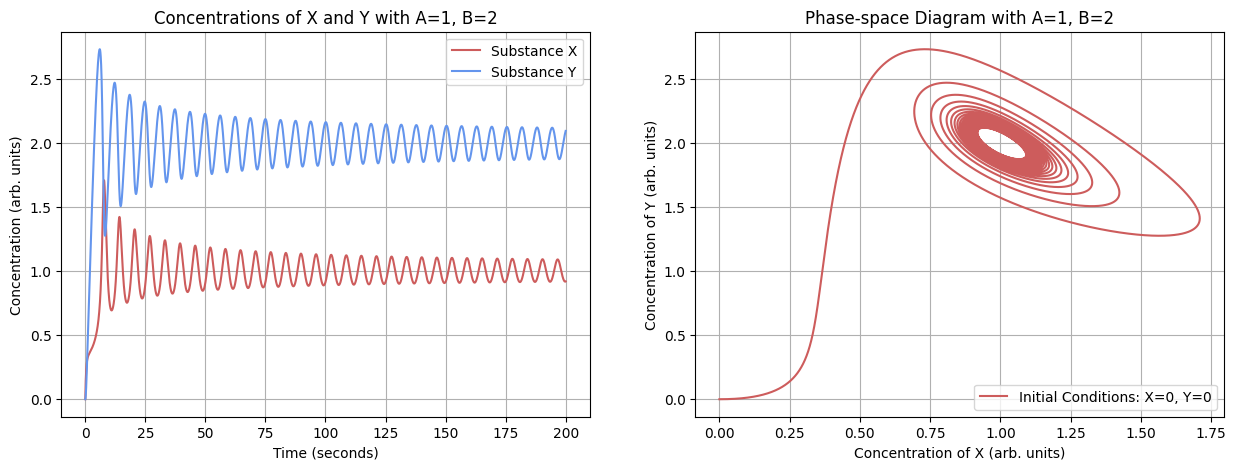
\includegraphics[width=2\columnwidth]{combinedPlot.png}
\caption{\label{fig:combinedPlot}Example caption}
\end{figure*}

\begin{figure*}
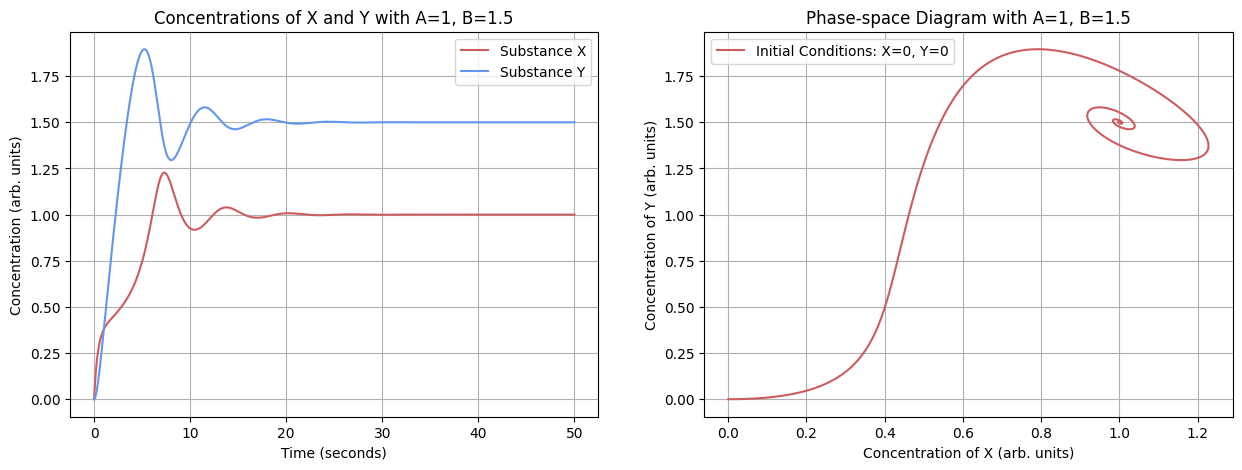
\includegraphics[width=2\columnwidth]{combinedPlot_fallToStable.png}
\caption{\label{fig:combinedPlot}Falls to stable point}
\end{figure*}

\begin{figure}
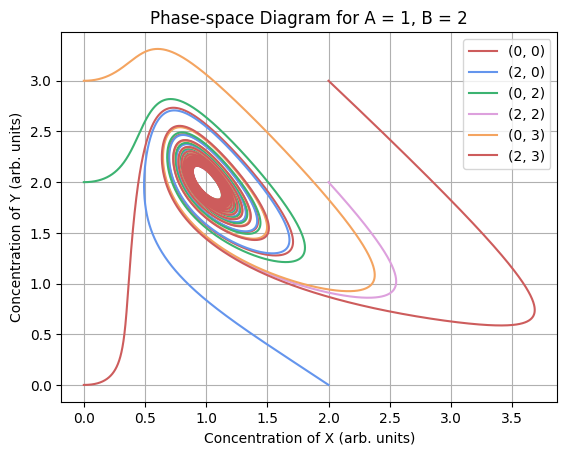
\includegraphics[width=0.85\columnwidth]{variationOfInitialConditions_phase.png}
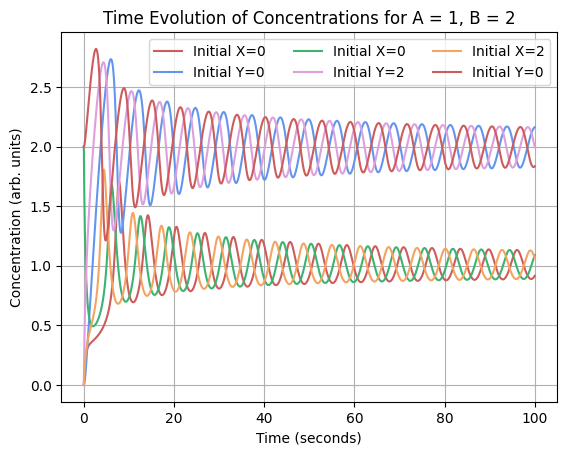
\includegraphics[width=0.85\columnwidth]{variationOfInitialConditions_evolution.png}
\caption{\label{fig:combinedPlot}Variation of initial conditions}
\end{figure}

\section{Conclusion}

\clearpage
\bibliography{chemOscillationsReferences.bib}

\clearpage

\section*{Appendix 1 - Derrivation of the Stable Point}
\begin{align*}
	\begin{aligned}
	A - (B + 1)X + X^2 Y &= 0\\
	BX - X^2 Y &= 0\\
	\\
	\therefore \hspace{1cm} X^2 Y &= BX\\
	\\
	\implies A - (B + 1)X + BX &= 0\\
	X &= A\\
	\\
	A^2 Y &= BA\\
	\implies Y &= \frac{B}{A}\\
	\\
	(X, Y) &= \left(A, \frac{B}{A}\right)
	\end{aligned}
\end{align*}

\end{document}



